\documentclass[a4paper, 12pt]{article}

\usepackage[margin=1.0in]{geometry}
\usepackage{amsmath}
\usepackage{amssymb}
\usepackage{graphicx}
\usepackage{hyperref}

\begin{document}

\title{Public-key criptography and the issues it faces with the emergence of quantum computers}
\author{Marko Vejnovi\'{c}}
\maketitle

\section{Rationale}
\paragraph*{}
As someone who is interested in computers, criptography has always piqued my interests. Although we use some sort of 
encryption almost every time we access the internet, my first interaction with cryptographic algorithms was when using 
the \textit{SSH} protocol.\footnote{The Secure Shell (SSH) Protocol is a protocol for secure remote login and other
secure network services over an insecure network. (Internet Requests for Comments, 2006)} The \textit{OpenSSH}
implementation can be configured to use different encryption algorithms, out which I found \textit{RSA}
\footnote{Rivest-Shamir-Adleman} to be the most interesting one, as it is by far the most commonly used one. Exploring
this algorithm sparked interest in me to further explore the field of cryptography, especially modern cryptography.

\section{Introduction}
\paragraph*{}
\textit{Cryptography} is the study of confidential communications in the presence of adversaries (Leeuwen, J. van.). 
The process of converting a readable message\footnote{Refered to as plaintext or cleartext.} into an undiscernable 
message\footnote{Refered to as ciphertext.} is called \textit{enciphering}, whereas the process of converting an 
enciphered message into readable form is refered to as \textit{deciphering} (ISO 7498-2:1989). The mathematical 
%TODO Fix citation
function which is used for enciphering and deciphering is called a \textit{cipher} (Schneier, Bruce). Usually these 
operations require different functions. A message $M$ is enciphered using the function $E$ to a ciphertext $C$.
$$E(M) = C$$
This ciphertext is then deciphered using $D$ back into $M$ again.
$$D(C) = M$$
Cryptography requires that the following must be true, as the essence of ciphers is being able to recover the original
plaintext (Schneier, Bruce):
$$D(E(M)) = M$$

\paragraph*{}
It is worth noting that characters, symbols or other similar notions are represented with numbers in the majority of 
cryptogrpahic systems.

\paragraph*{}
Historically, two types of ciphers existed - restricted ciphers and key ciphers. The former relied on adversaries not 
knowing the cipher itself. Restricted ciphers have almost completely vanished from use, as they present many issues - 
no quality control, no standardization, modern computers being able to crack such types of ciphers only being a few of 
%TODO Replace word crack with something more professional
them (Schneier, Bruce). The earliest of ciphers, such as the Atba\v{s} cipher were, indeed, restricted ciphers. Key 
ciphers present themselves as a solution to these issues. Both enciphering and deciphering is done using a key:
$$E_k(M) = E(M, k) = C$$
$$D_k(C) = D(C, k) = M$$

For the majority of the history of cryptography, \textit{symmetric ciphers} were employed. Symmetric ciphers are 
ciphers where the same key for enciphering and deciphering must be used.
$$E_k(M) = C$$
$$a \neq k \implies D_k(C) \neq M$$

One of the first noted uses of a symmetric key cipher was the \textit{Caesar's cipher}. It, among other substitution 
ciphers, shifted a character in the alphabet to another by the key:
%TODO Phrase this better
$$C = M + k$$
$$M = C - k$$

Other similar, more complex, systems have emerged throughout history, however, they all shared a common issue - they 
key was required to be transmitted in secrecy.

Until 1976, with the publication of \textit{New Directions in Cryptography} by Whitfield Diffie and Martin E. Hellman, 
the key was necessary to be transmitted in secrecy\footnote{Actually, this paper was preceeded by James Ellis's work 
(1975), however, Ellis's work remained top secret in the \textit{Goverment Communications Headquarters} until 1997, 
when it was fully released to the public (Sawer, Patrick).}. The work of this paper resulted in an algorithm which 
allowed for transmitting a key in public, called the \textit{Diffie-Hellman key exchange}. \textit{New Directions in 
Cryptography} is the paper with which modern cryptography starts.

The Diffie-Hellman key exchange does however, have two issues. The first is that there is a need for a courier to 
actually transmit the key (although the courier does not know what the key is). The second issue is that the listening 
party has no way of knowing if a message sent was sent by the expected party.

\paragraph*{}
\textit{Public-key ciphers} present themselves as a solution to both of these issues. Public-key ciphers are ciphers 
which operate by using different keys for enciphering and deciphering.
$$C = E_{k1}(M)$$
$$M = D_{k2}(C)$$
These ciphers are called "public-key" because the enciphering can be done in public. The enciphering key is called the 
\textit{public key}, whereas, the deciphering key is denoted to as the \textit{private key}. Anyone is able to enipher 
a message using the public key, but only specific people are able to decipher it with their private key. The most 
widely known, and most widely used public-key cipher is the \textit{RSA}\footnote{Rivest-Shamir-Adleman} 
cipher\footnote{The paper \textit{A Method For Obtaining Digital Signatures And Public-Key Cryptosystems} was published
 by Rivest, R. L. et al. in 1977.}.

\paragraph*{}
Both of these ciphers are based on modular arithmetic. For analyzing how well different algorithms perform, the notion 
of time complexity is used\footnote{Time complexity is a measure of the time taken to perform a certain algorithm in 
terms of individual instructions. It is the number of instructions required $O(n)$ to perform on input whose size is 
$n$. To exemplify, a function which searches for an element in an array of length $n$ takes $n$ instructions to 
perform - for every element of the array, a check is done to see whether the element is the one that is searched for.}.

\section{Modular arithmetic}

\subsection{Introduction}
\paragraph*{}
It was Gauss who gave the modern definition of modular arithmetic: If a number $m$ divides the difference of the 
integers $b$ and $c$\footnote{These integers can be positive or negative, they are taken absolutely, unsigned.}, 
$b$ and $c$ are \textit{congruent relative} to $m$, otherwise, they are \textit{noncongruent}. The number $m$ is 
defined as the \textit{modulus} (Gauss, Carl Friedrich). If the numbers $b$ and $c$ are, indeed, congruent, they are 
called a \textit{residue} of the other.

\paragraph*{}
For a number $a$, all of its residues modulo $m$ are contained in the formula
$$a + km$$
where k is any integer (Gauss, Carl Friedrich).

\paragraph*{}
Gauss also introduced the modern congruence notation\footnote{It is worth noting that Gauss in reality wrote the 
modulus in parenthesees $$a \equiv b \pmod{m}$$ but for the purposes of this paper, I will use the more modern, also 
widely accepted, parenthesees-less notation.}:
$$a \equiv b \mod m$$

\paragraph*{}
To exemplify the previous statements:
$$5 \equiv 28 \mod 23$$
$5$ is congruent to $28$ modulo $23$ means the following:
\begin{gather*}
  \lvert 28 - 5 \rvert = 23 \cdot k\\
  \text{where } k \in \mathbb{Z}
\end{gather*}
This also means that the remainder of integer division between $28$ and $23$ is $5$. Some textbooks explain modular 
arithmetic as an arithmetical system where values "wrap around" upon reaching the modulus value. This is often 
exemplified with the idea of a clock: the hour hand is congruent relative to modulo $12$, the minute and second hands 
are congruent relative to $60$.

\subsection{Properties}
% TODO

\section{The \textit{Diffie-Hellman key exchange}}
\paragraph*{}
The \textit{Diffie-Hellman key exchange}, as applied as it is today, is mathematically not complex. The name ``key 
exchange" is a misnomer, however, as this algorithm does not actually exchange keys between communicators, rather, the 
communicators generate the same key.

\paragraph*{}
Suppose that you have two people, $a$ and $b$. They are in the presence of an adversary $e$. $a$ and $b$ have their 
%TODO Replace word people
private spaces in which they are able to store information safely, however, in order for them to communicate any piece 
of data, it must go through a public space which $e$ has access to. The \textit{Diffie-Hellman key exchange} works as 
follows.
First, $a$ and $b$ agree on two shared constants, $q$ and $n$. $q$ is a relatively small prime integer, whereas $n$ is 
%TODO Figure out why the fuck q is prime
a big integer\footnote{Today, the value of $n$ most commonly used is around $10^{1200}$.}. These are communicated via 
the public space and $e$ also knows these values. $a$ and $b$ then randomly choose a value $x_a$ and $x_b$ such that 
$$0 < x < n$$, and these values are kept private and not shared. Both of these people now calculate the value
%TODO Replace word people
$$Y = q^x \mod n$$
These result in $Y_a$ and $Y_b$. $Y_a$ and $Y_b$ are then shared to the public space. $a$ and $b$ now calculate
 $K_a$ and $K_b$ as follows:
$$K_a \equiv Y_b^{x_a} \mod n \Longleftrightarrow (q^{x_b} \mod n)^{x_a} \mod n \Longleftrightarrow q^{x_b x_a} \mod n$$
$$K_b \equiv Y_a^{x_b} \mod n \Longleftrightarrow (q^{x_a} \mod n)^{x_B} \mod n \Longleftrightarrow q^{x_a x_b} \mod n$$
%TODO Reference a property of modular arithmetic
These values of $K_a$ and $K_b$ are equal and used as the common key for further symmetric enciphering. $e$ is unable 
to calculate $K$ without knowing either $x_a$ or $x_b$.

\paragraph*{}
In order for $e$ to calculate an $x$ he must perform the following calculation:
$$X = log_q Y \mod n$$
This issue is named the \textit{discrete logarithm}.

\paragraph*{}
It is precisely because of this why the \textit{Diffie-Hellman key exchange} is cryptographically secure. The 
computation time required for calculating the discrete logarithm, with today's algorithms, at best is $\sqrt{n}$.
%TODO Which algorithm
%TODO Show why
The computational time required for calculating $Y$ from $x$ is at worst $2log_2 q$ (Diffie, W., and M. Hellman).
%TODO Show why

\paragraph*{}
In figure \ref{fig:n-xy-time}, the relationship between the difference of time required to generate $Y$ and the time 
to perform a discrete logarithm in order to calculate $x$, as performed by a simulation\footnote{The simulation was 
written in \textit{python} and the data was plotted using \textit{matplotlib}. The exact code is published online at 
the following link: INSERT-LINK.}\footnote{The outlier at is most likely due to incorrect time measurements by the 
system. Reference the original code for more information as to why this might've ocurred.}.
%TODO Insert link
\begin{figure}[ht]
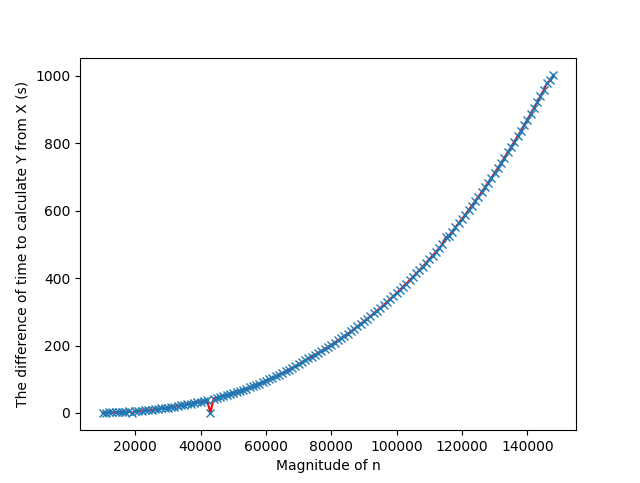
\includegraphics[width=12cm]{n_xy-time_relationship}
\centering
\caption{The relationship between the magnitude of $n$ and the difference of time required to calculate $X$ from $Y$ 
and $X$ using a \textit{brute-force} $X$ calculation algorithm.}
\label{fig:n-xy-time}
\end{figure}

\pagebreak
\begin{thebibliography}{9}
\bibitem{rfc4251}
Ylonen, T. \textit{The Secure Shell (SSH) Protocol Architecture}. Internet Requests for Comments. Edited by Lonvick, C.
The Internet Society, 2006.
\bibitem{sshd_man}
\textit{sshd\_config(5) Linux User's Manual}. 2006.
\bibitem{cs_handbook}
Leeuwen, J. van. \textit{Handbook Of Theoretical Computer Science}. Elsevier Science Publishers, 1990, p. 719.
%TODO Add ISO 7498-2:1989 citation
\bibitem{applied_cryptography}
Schneier, Bruce. \textit{Applied Cryptography, Second Edition: Protocols, Algorthms, And Source Code In C}. 2nd ed., John Wiley \& Sons, Inc., 1996.
\bibitem{cripto_history}
\textit{A Brief History of Cryptography}. http://cryptozine.blogspot.com/2008/05/brief-history-of-cryptography.html
\bibitem{ellis_newspaper}
Sawer, Patrick. ``\textit{The Unsung Genius Who Secured Britain's Computer Defences and Paved the Way for Safe Online Shopping.}'' The Telegraph, 11 Mar. 2016.
\bibitem{rsa}
Rivest, R. L. et al. ``\textit{A Method For Obtaining Digital Signatures And Public-Key Cryptosystems}''. 1977, Accessed 27 Mar 2018.
\bibitem{disqutiones}
Gauss, Carl Friedrich. \textit{Disquisitiones Arithmeticae}. Yale University, 1966.
\bibitem{dh_key_exchange}
Diffie, W., and M. Hellman. ``\textit{New Directions in Cryptography.}'' IEEE Transactions on Information Theory, vol. 22, no. 6, 1976, pp. 644–654., doi:10.1109/tit.1976.1055638.
\bibitem{python}
Python Software Foundation. \textit{Python Language Reference}, version 2.7. Available at \url{http://www.python.org}
\bibitem{matplotlib}
Hunter, J. D. \textit{Matplotlib: A 2D graphics environment}. Computing In Science \& Engineering, vol. 9, no. 3, 2007, pp. 90-95., doi:10.1109/MCSE.2007.55
\end{thebibliography}

\end{document}
